\documentclass[border=4pt]{standalone}
% Shared typography and colours for the standalone figures.
\usepackage{unicode-math}
\setmainfont{TeX Gyre Termes}
\setmathfont{TeX Gyre Termes Math}
\usepackage{tikz}
\usetikzlibrary{arrows.meta,positioning,calc,decorations.pathreplacing}
\usepackage{pgfplots}
\pgfplotsset{compat=1.18}

% One colour per element or subsystem. Record the mapping in
% the working repository conventions and use it identically in every figure.
\definecolor{elemA}{HTML}{1F5FA8}
\definecolor{elemB}{HTML}{B8461B}
\definecolor{elemC}{HTML}{2E7D32}
\definecolor{elemD}{HTML}{6A4C93}
\definecolor{frameline}{HTML}{555555}

% Article-specific diagram styling; common figure-style.tex remains managed.
\usepackage{circuitikz}
\usetikzlibrary{decorations.pathmorphing,fit,backgrounds}
\tikzset{
  every node/.style={font=\small},
  block/.style={draw=frameline,rounded corners=2pt,minimum height=7mm,align=center,fill=white},
  massA/.style={draw=elemA,fill=elemA!10,thick},
  massB/.style={draw=elemB,fill=elemB!10,thick},
  receiver/.style={draw=elemC,fill=elemC!9,thick},
  mediator/.style={draw=elemD,fill=elemD!8,thick},
  flow/.style={-{Latex[length=2.3mm]},thick},
  boundary/.style={draw=frameline,dashed,rounded corners=3pt},
  spring/.style={decorate,decoration={coil,aspect=.4,segment length=3mm,amplitude=1.5mm},thick,elemD}
}

\begin{document}
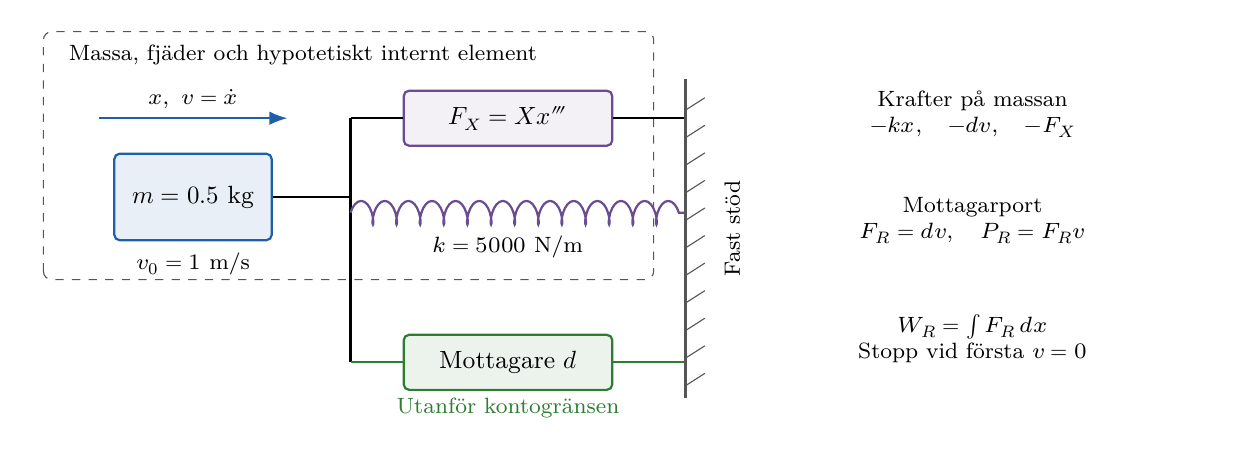
\begin{tikzpicture}
\path[use as bounding box] (0,-1.5) rectangle (15,3.55);
\draw[boundary] (.2,.35) rectangle (7.95,3.5);
\node[font=\footnotesize,anchor=west] at (.4,3.2) {Massa, fjäder och hypotetiskt internt element};
\node[block,massA,minimum width=2cm,minimum height=1.1cm] (m) at (2.1,1.4) {$m=0.5$ kg};
\draw[flow,elemA] (.9,2.4)--(3.3,2.4);
\node[above,font=\footnotesize] at (2.1,2.4) {$x,\ v=\dot x$};
\node[font=\footnotesize] at (2.1,.55) {$v_0=1$ m/s};
\draw[thick] (m.east)--(4.1,1.4);
\draw[thick] (4.1,-.7)--(4.1,2.4);
\node[block,mediator,minimum width=2.65cm] (x) at (6.1,2.4) {$F_X=Xx'''$};
\draw[thick] (4.1,2.4)--(x.west);
\draw[thick] (x.east)--(8.35,2.4);
\draw[spring] (4.1,1.2)--(8.35,1.2);
\node[below,font=\footnotesize] at (6.1,1.03) {$k=5000$ N/m};
\node[block,receiver,minimum width=2.65cm] (r) at (6.1,-.7) {Mottagare $d$};
\draw[thick,elemC] (4.1,-.7)--(r.west);
\draw[thick,elemC] (r.east)--(8.35,-.7);
\node[below,font=\footnotesize,text=elemC] at (6.1,-1.03) {Utanför kontogränsen};
\draw[very thick,frameline] (8.35,-1.15)--(8.35,2.9);
\foreach \h in {-1,-.65,...,2.85}
  \draw[frameline] (8.35,\h)--(8.6,\h+.16);
\node[font=\footnotesize,rotate=90] at (8.95,1) {Fast stöd};
\node[font=\footnotesize,align=center] at (12,2.45)
  {Krafter på massan\\$-kx,\quad-dv,\quad-F_X$};
\node[font=\footnotesize,align=center] at (12,1.1)
  {Mottagarport\\$F_R=dv,\quad P_R=F_Rv$};
\node[font=\footnotesize,align=center] at (12,-.4)
  {$W_R=\int F_R\,dx$\\Stopp vid första $v=0$};
\end{tikzpicture}
\end{document}
